\documentclass[12pt,a4paper,oneside]{book} 

%%%%%%%%%%%%%%%%%%%%%%%%%%%%%%%%%%%%%%%%%%%%%%%%%%%%%%%%%%%%%%%%%%%%%%%%

\usepackage{ifthen}
\usepackage{graphicx}
\usepackage[dvips]{epsfig}
\usepackage{enumerate}
\usepackage{calc}
\usepackage{multicol} 
\usepackage{titlesec}
%\usepackage{showkeys}
\usepackage{comment}
\usepackage{mathtools}
%%%%%%%%%%%%%%%%%%%%%%%%%%%%%%%%%%%%%%%%%%%%%%%%%%%%%%%%%%%%%%%%%%%%%%%%
\usepackage[version=3]{mhchem}
\usepackage{a4}
\usepackage{amsfonts}
\usepackage{amssymb}
\usepackage{epsfig}

%%%%%%%%%%%%%%%%%%%%%%%%%%%%%%%%%%%%%%%%%%%%%%%%%%%%%%%%%%%%%%%%%%%%%%%%

\usepackage{t1enc,times}
\usepackage{latexsym,amssymb}
\usepackage{amsmath}
\usepackage{amstext}

\usepackage{amssymb}
%\usepackage[T1]{fontenc}
%\usepackage{cmbright}
\usepackage{pifont}
\usepackage{marvosym}
%\usepackage{pslatex}
\usepackage{stmaryrd}
%\usepackage{txfonts}  

%%%%%%%%%%%%%%%%%%%%%%%%%%%%%%%%%%%%%%%%%%%%%%%%%%%%%%%%%%%%%%%%%%%%%%%%%%%%%%%

\usepackage{fancybox} 
\usepackage{fancyhdr}
\usepackage{fullpage}

%%%%%%%%%%%%%%%%%%%%%%%%%%%%%%%%%%%%%%%%%%%%%%%%%%%%%%%%%%%%%%%%%%%%%%%%%%%%%%%

%\usepackage{url}    
%\ExecuteOptions{dvips}
%\usepackage[pdftex,colorlinks=true]{hyperref}
%\hypersetup{backref,pdfpagemode=UseThumbs,pdfstartview=Fit,
%pdfpagelayout=SinglePage,pdfstartpage=1,colorlinks=true,menucolor=msc,
%anchorcolor=msc,pagecolor=msc,urlcolor=rfr,breaklinks=true,hyperfootnotes=true}

%%%%%%%%%%%%%%%%%%%%%%%%%%%%%%%%%%%%%%%%%%%%%%%%%%%%%%%%%%%%%%%%%%%%%%%%%%%%%%%

\pagestyle{fancy}
\fancyhf{} 
%\renewcommand{\headrulewidth}{1pt}
%\renewcommand{\footrulewidth}{1pt}
\renewcommand{\headwidth}{\textwidth}
\fancyhead[LE]{\leftmark}
\fancyhead[RO]{\small \rightmark}
\fancyfoot[C]{\thepage}

%%%%%%%%%%%%%%%%%%%%%%%%%%%%%%%%%%%%%%%%%%%%%%%%%%%%%%%%%%%%%%%%%%%%%%%%%%%%%%%

\tolerance 4000
\textwidth 17.00cm
\topmargin -0.30cm
\oddsidemargin -0.25cm
\evensidemargin -0.25cm
\textheight 23.00cm
%\headsep 12pt
\headheight 15pt
\footskip 60pt
%\parindent 12pt

%%%%%%%%%%%%%%%%%%%%%%%%%%%%%%%%%%%%%%%%%%%%%%%%%%%%%%%%%%%%%%%%%%%%%%%%%%%%%%%

\renewcommand{\rmdefault}{ptm}  % times
\renewcommand{\rmdefault}{phv}  % helvetica
\renewcommand{\rmdefault}{pbk}  % bookman
\renewcommand{\rmdefault}{ppl}  % palatino
\renewcommand{\sfdefault}{phv}  % helvetica as sans serif
\renewcommand{\ttdefault}{pcr}  % courier as fixed width
\renewcommand{\tabcolsep}{8pt}
\renewcommand{\arraystretch}{1.25}

%%%%%%%%%%%%%%%%%%%%%%%%%%%%%%%%%%%%%%%%%%%%%%%%%%%%%%%%%%%%%%%%%%%%%%%%%%%%%%%

\def\nn{\nonumber}
\def\f{{\frac}}
\def\pa{{\partial}}
\def\d{{\rm d}}
\def\l{\left}
\def\r{\right}
\def\Mpl{M_{_{\rm Pl}}}

%%%%%%%%%%%%%%%%%%%%%%%%%%%%%%%%%%%%%%%%%%%%%%%%%%%%%%%%%%%%%%%%%%%%%%%%%%%%%%%

\def\done{\marginpar {\scriptsize DONE}}
\def\check{\marginpar {\scriptsize CHECK}}

%%%%%%%%%%%%%%%%%%%%%%%%%%%%%%%%%%%%%%%%%%%%%%%%%%%%%%%%%%%%%%%%%%%%%%%%%%%%%%%

\begin{document}

%%%%%%%%%%%%%%%%%%%%%%%%%%%%%%%%%%%%%%%%%%%%%%%%%%%%%%%%%%%%%%%%%%%%%%%%%%%%%%%

\baselineskip 20pt

%%%%%%%%%%%%%%%%%%%%%%%%%%%%%%%%%%%%%%%%%%%%%%%%%%%%%%%%%%%%%%%%%%%%%%%%%%%%%%%

\pagenumbering{roman}

%%%%%%%%%%%%%%%%%%%%%%%%%%%%%%%%%%%%%%%%%%%%%%%%%%%%%%%%%%%%%%%%%%%%%%%%%%%%%%%

\thispagestyle{empty}
\topskip 45pt
%\hrule\hrule\hrule\hrule\hrule

\vskip 30pt
\centerline{ \Huge Notes on Astroparticle Physics} 
\vskip 25pt
\centerline{\Large  S.Sindhu Sri Sravya}
\vskip 8pt
\vskip 30pt 
%\begin{center}
%
\epsfig{file=iitm.ps, width=3.0cm, height=3.0cm}
%\begin{figure}[h]
 %   \centering
  %  
\includegraphics[width =3.0cm,height=3.0cm]{iitm.jpg}
    %\caption{Caption}
    %\label{fig:my_label}
%\end{figure}
%\end{center}
\vskip 8pt 
\centerline{\Large  Department of Theoretical Physics}
\vskip 8pt 
\centerline{\Large  Tata Institute of Fundamental Research}
\vskip 8pt 
\centerline{\Large  Mumbai 400005}
\vskip 8pt
%\centerline{\Large \bf April~2012}
%%%%%%%%%%%%%%%%%%%%%%%%%%%%%%%%%%%%%%%%%%%%%%%%%%%%%%%%%%%%%%%%%%%%%%%%%%%%%%%



%%%%%%%%%%%%%%%%%%%%%%%%%%%%%%%%%%%%%%%%%%%%%%%%%%%%%%%%%%%%%%%%%%%%%%%%%%%%%%%

\newpage
\thispagestyle{empty}
\tableofcontents
\newpage

%%%%%%%%%%%%%%%%%%%%%%%%%%%%%%%%%%%%%%%%%%%%%%%%%%%%%%%%%%%%%%%%%%%%%%%%%%%%%%%

\pagenumbering{arabic}

%%%%%%%%%%%%%%%%%%%%%%%%%%%%%%%%%%%%%%%%%%%%%%%%%%%%%%%%%%%%%%%%%%%%%%%%%%%%%%%

\chapter{Introduction to Cosmology}
\section{ Outline}

\section{Overview}
\subsection{Model for the universe}
\subsection{Support for bigbang theory}
Hubble diagram, light element abundances, CMB
\subsection{Notations and Conventions}
\subsubsection{Natural units}
\subsubsection{ metric sign convention}
\section{FLRW Metric}
For a homogeneous and isotropic universe, which is expanding, the invariant spacetime interval is \begin{equation}
    ds^2 = dt^2 - a(t)^2(\frac{dr^2}{1-kr^2} -r^2d\Omega^2)
\end{equation}
where $d\Omega^2 = d\theta^2 + sin^2\theta d\phi^2$ and k is the spatial curvature
\newline This apparent "distance" between two space-time events is expressed in terms of the metric, which depends on the geometry of space-time. The space part of the metric can be understood in analogy to how distances in 2D are measured. The expression for distance between two points on the surface of a plane sheet is different from that of a spherical surface. On a plane, the distance can be written using Cartesian co-ordinates as:
\begin{equation}
    dl^2 = dx^2+dy^2
\end{equation}
While on the sphere, the distance in polar co-ordinates is :
\begin{equation}
    dl^2 = R^2d\theta^2 + R^2sin^2\theta d\phi^2
\end{equation}
 where R is the radius of the 3 dimensional sphere thought of as embedding the 2D surface. \textbf{Note that it is not possible to represent the distance between two points on a sphere in the same form as Eq(1.2) i.e; the co-effecients of $d\theta^2$ and $d\phi^2$ are not constants and it cannot be expressed in such a form, since the surface is intrinsically "curved"}. Curvature of any curve is defined as the rate of change of its slope.Therefore, we can expect the curvature of space-time to be a function of the second derivative of metric. A sphere by definition is negatively curved , while a hyperbolic surface is positively curved and the curvature of a flat surface is evidently zero.   
\par \noindent Eqn(1.3) can also be represented as follows.
\begin{equation}
    ds^2 = dx_{1}^2 +dx_{2}^2 + dx_{3}^2
\end{equation}
where $x_{1}^2 +x_{2}^2+x_{3}^2 = R^2 $ and therefore $x_{3}^2 = R^2 - x_{1}^2-x_{2}^2$. Differentiating this equation and substituting $x_{1} = rsin\theta $ and $x_{2} = rcos\theta$, we have 
\begin{equation}
    ds^2 =  \frac{R^2dr^2}{R^2-r^2} +r^2 d\theta^2
\end{equation}
which can be re-scaled to r' = r/R and therefore , we have 
\begin{equation}
    ds^2 = R^2(\frac{dr'^2}{1-r'^2} + r^2d\theta^2) 
\end{equation}
This is the distance on a 2D surface. Similarly, we can imagine a 3D surface as enclosing a sphere in the 4 dimensions. The equation for this sphere would be 
\begin{equation}
    x_{1}^2 +x_{2}^2+x_{3}^2 +x_{4}^2 = R^2
\end{equation}
\begin{equation}
   \therefore x_{4}^2 = R^2 - x_{1}^2-x_{2}^2 -x_{3}^2
\end{equation}
and the line element is 
\begin{equation}
    dl^2 = dx_{1}^2 +dx_{2}^2 + dx_{3}^2 + dx_{4}^2
\end{equation}
Differentiate Eqn(1.8) to substitute in Eqn(1.9) and using spherical polar coordinates, we have
\begin{equation}
    dx_{1}^2 +dx_{2}^2 + dx_{3}^2 + dx_{4}^2 = R^2(\frac{dr^2}{1-r^2}+r^2d\theta^2+r^2sin^2\theta d\phi^2)
\end{equation}
Now, we have the spacetime line interval 
\begin{equation}
    ds^2  = g_{\mu\nu}dx^{\mu}d^{\nu}
\end{equation}
Applying the principle of homogeneity and isotropy, we can elimante the $g_{0i}$ terms since the cross terms violate isotropy. The most general spatial metric will then be the expression (1.10) we derived above, for a closed universe. Therefore, in general, the FLRW metric is given as 
\begin{equation}
      ds^2 = dt^2 -a(t)^2(\frac{dr^2}{1-kr^2}+r^2d\theta^2+r^2sin^2\theta d\phi^2)
\end{equation}
where we have R: radius of the 4-sphere as the scale factor a(t)(Imagine the radius of the 4 sphere changing with time) and k is the spatial curvature: +1 for closed universe, -1 for open and 0 for flat universe. 
\section{Particle Kinematics}
\section{Defining distances in Cosmology}
One has to be careful while talking about distances in Cosmology, since the space in which we live is itself expanding. Defining comoving coordinates as the co-ordinate system in which the universe is static at all times everywhere, we can write physical distance r as:
\begin{equation}
    r = a x
\end{equation}
where a is the scale factor and x is the comoving coordinate. Special relativity postulates that information cannot be transferred at a rate faster than the speed of light in vacuum. Therefore, for each point in space time, the maximum distance from which it could have received a signal will be :
\begin{equation}
    d = c*r_{c}
\end{equation}
where $r_{c}$ is the comoving distance travelled by light since bigbang until reaching us today. This distance can be computed since we know that the trajectory of light is given by:
\begin{equation}
    ds^{2} = 0
\end{equation}
Using the FLRW metric,
\begin{equation}
    dt^{2} = a^{2}(t)(dx^2+dy^2+dz^2)
\end{equation}
if light is emitted radially in all directions,
\begin{equation}
    \frac{dt^2}{a(t)^2} = dr_{c}^2
\end{equation}
Integrating, we get
\begin{equation}
    r_{H}  = \int_{t_{em}=0}^{t_{0}} \frac{dt}{a(t)}
\end{equation}
$r_{H}$ is called the cosmological horizon.
\subsection{Redshift}
As the universe is expanding, the physical wavelength changes with the scale factor as we have seen above. This phenomenon is called redshifting, since larger wavelengths are "redder". The amount by which any wavelength increases/decreases is given by :
\begin{equation}
    1+z = \frac{\lambda_{obs}}{\lambda_{em}} = \frac{a_{0}}{a(t)}
\end{equation}
where z is called the cosmological redshift, different from the Doppler redshift because it is due to the expansion of the Universe or the scale factor a(t), unlike because of moving sources in the case of Doppler shift.
\\We can measure distances to astrophysical objects by looking at them, and if we know how the path of the light it emitted gets changed before reaching us, we can decide how far the object should have been. The other way is by looking at its apparent size and comparing to the actual size to estimate how far it is. The following sections discuss how these distances are measured.
\subsection{Luminosity distance}
Consider a source emitting light in all directions. In a given comoving volume, the total energy emitted should be constant. The total energy emitted per unit area per unit time is called the flux.  
\begin{equation}
    F_{obs} = \frac{L(r)}{4\pi a(t_{0}^2)r^2}
\end{equation}
where L(r) is the luminosity at a comoving distance r from the source. The absolute luminosity of a source is the energy it emits per unit time. In an expanding universe, as the emitted light reaches the observer, the luminosity decreases by factor of $(1+z)^2$ because the wavelength of emitted light gets redshifted by a factor of (1+z) and the time between two successive waves gets delayed by factor of (1+z).The luminosity at our location is therefore
\begin{equation}
L(r) = \frac{L}{(1+z)^2}    
\end{equation}
where L is the absolute luminosity of the source. The flux observed is therefore 
\begin{equation}
    F_{obs} = \frac{L}{4\pi d_{L}^2}
\end{equation}
where 
\begin{equation}
    d_{L} = a(t_{0})r(1+z)
\end{equation}
$d_{l}$ is called the luminosity distance. If we some how know the intrinsic luminosity of a source and measure the flux from it, we know the distance $d_{L}$ to the object. The sources for which absolute luminosity is known are termed as Standard candles.
\\ The luminosity distance for nearby sources can be found out as follows. In a flat universe, assuming that light rays are travelling towards us radially, we have
\begin{equation}
    r = \int_{t_{em}}^{t_{0}}\frac{dt}{a(t)} 
\end{equation}
If we are not looking too far, i.e; if $t_{em} = t_{0} - \Delta t $. The scale factor can be taylor expanded into
\begin{align}
    a(t)  &= a(t_{0}) + (t-t_{0}) \Dot{a(t)}|_{t_{0}} + .....\nonumber\\
   \implies a(t) &=  a(t_{0})(1+ H_{0}(t-t_{0}))
\end{align}
The integral, upto first order in time will therefore be 
\begin{align}
    r  &= \int_{t_{em}}^{t_{0}}\frac{dt}{a(t_{0})(1+H_{0}(t-t_{0}))}\nonumber\\
      &= \int_{t_{em}}^{t_{0}}\frac{dt}{a(t_{0})}(1-H_{0}(t-t_{0}))\nonumber\\
      &= -\frac{t_{em}-t_{0}}{a_{0}}
\end{align}
In terms of redshift, we have
\begin{equation*}
   \frac{1}{1+z} =  1-z = \frac{a(t)}{a(t_{0})}  \approx 1 - H_{0}(t_{em}-t_{0})
\end{equation*}
\begin{equation}
    \therefore z \approx H_{0}(t_{em} - t_{0})
\end{equation}
Substituting back, we get
\begin{equation}
    r = \frac{z}{a_{0}H_{0}}
\end{equation}
The luminosity distance will be 
\begin{equation*}
    d_{L} = a(t_{0})(1+z)(z)*\frac{1}{a_{t_{0}}H_{0}} 
\end{equation*}
Therefore, upto first order, we have 
\begin{equation}
    d_{L} \approx H_{0}^{-1} z
\end{equation}
The above equation is stated as the Hubble's law. *Hubble history - verify* Edwin Hubble had observed that the spectra of all nearby galaxies were redshifted by an amount proportional to their distance from us. The proportionality constant is called the Hubble's constant and was first calculated to be ?? . It is evident that the better the measurement of distance $d_{l}$, the better the value of Hubble's constant today. This approach is a direct way to calculate the Hubble's constant today. There are other indirect ways to calculate the Hubble's constant, for example, from the CMB spectrum.??    
\subsection{Angular diameter distance}
Consider a source of proper diameter D, emitting light. The angular size(for small angles) of the source is 
\begin{equation}
    \delta \theta = \frac{D}{d_{A}}
\end{equation}
where $d_{A}$ is the angular diameter distance, which is just equal to 
\begin{equation}
    d_{A} = ra(t_{em}) = \frac{r}{1+z}
\end{equation}
where r is the comoving distance from the source, given by \textbf{Eq(1.24)}.

\section{Friedmann Equations}
The Einsteins field equations for gravity are :
\begin{equation}
    G_{\mu\nu} = 8\Pi GT_{\mu\nu}
\end{equation}
where $ G_{\mu\nu} = R_{\mu\nu} - \frac{1}{2} g_{\mu\nu}R $ and $T_{\mu\nu}$ is the stress energy tensor.
\par The expanding, homogeneous and isotropic universe is described by the FLRW metric and the Christtoffel symbols for this metric was derived in Sec(1.3). The non-zero components of curvature tensor can therefore be calculated to be :
\begin{align}
    R_{00} &= -3\frac{\Ddot{a}}{a}\\
    R_{ij} &= -g_{ij}(\frac{\Ddot{a}}{a}+2\frac{\dot{a}^2}{a^2}+2\frac{k}{a^2}) 
\end{align}
and the Ricci scalar is :
\begin{equation}
    R = -6 (\frac{\Ddot{a}}{a}+\frac{\dot{a}^2}{a^2}+\frac{k}{a^2})  
\end{equation}
The Einstein tensor is therefore:
\begin{align}
    G_{00} &= \frac{\dot{a}^2}{a^2}+\frac{k}{a^2} \\
    G_{ij} &= \delta_{ij}(\frac{2\Ddot{a}}{a}+\frac{\dot{a}^2}{a^2}+\frac{k}{a^2}) 
\end{align}
\subsection{Stress Energy Tensor}
Imagine particles moving across in a box randomly with different velocities. The stress energy tensor can then be thought of as describing the second moment of the velocity distribution at any given location.  
\begin{equation}
     T_{ij} \propto \int n_{0}v_{i}v_{j}f(v)d^3v
\end{equation}
where $n_{0}$ is the number density of particles, $v_{i,j}$ velocities of i th and j th particles, f(v) is the distribution function of velocities.**** It can be seen that the stress-energy tensor is symmetric. The $T_{00}$ component is the energy density, $T_{0i}$ components represent flux of i th component of momentum along time?? , while $T_{ii}$ and $T_{ij}$ components correspond to pressure($\propto v^2$ ) and shear stress(or flux of i th component of momentum along j th direction).\\
We assume that the universe is covered in a perfect fluid i.e; fluid with no viscosity, shear stress and doesn't conduct heat. In the comoving frame, the stress energy tensor can therefore be written as 
\begin{equation}
    T_{\mu\nu} = diag(\rho,-p,-p,-p)
\end{equation}
where $\rho$ is the energy density and p is the pressure, which are related to each other by an equation of state.
Plugging into the Einsteins equations, we get :
\begin{align}
    \frac{\dot a^2}{a^2} + \frac{k}{a^2} &= \frac{8\pi G \rho}{3} \\
    2 \frac{\Ddot{a}}{a} + \frac{\dot a^2}{a^2} + \frac{k}{a^2} &= -8 \pi G p
\end{align}
\subsection{Density parameters}
The Friedmann equations shown above can be re-written in a form such that they are in terms of observable parameters, the density parameters. For the first equation, the LHS term $\frac{\dot{a}}{a} = H$, is the Hubble parameter.On the RHS, the density and pressure for different components(R- relativistic,NR- non-relativistic,$\Lambda$- Dark energy/Cosmological constant) of the Universe can be written as:
\begin{equation}
    \rho(t) = \rho_{R}^{0}(\frac{a_{0}}{a})^4 + \rho_{NR}^{0}(\frac{a_{0}}{a})^3 + \rho_{\Lambda}
\end{equation}
where subscript 0 indicates quantities as seen today.The energy density of non-relativistic matter should remain constant in a given comoving volume, therefore as the physical volume increases as $a^3$, the energy density falls off as $1/a^3$. For relativistic species or radiation, in addition to the increase in volume, the energy also falls of by a factor of a(t), since the physical wavelength increases with a(t). Therefore, the radiation energy density goes as $1/a^4$. The energy density of dark energy is constant(it was introduced as the cosmological constant) and its origins are discussed in \footnote[reference]. 
\\We'll consider the universe to be flat, so that k = 0\footnote{Explain why its a reasonable thing to do}. The eqn(1.40) then becomes
\begin{equation}
    H^2 = \frac{8\pi G }{3}[\rho_{R}^{0}(\frac{a_{0}}{a})^4 + \rho_{NR}^{0}(\frac{a_{0}}{a})^3 + \rho_{\Lambda}]
\end{equation}
Different epochs: As we can see from the equation, at early times the $\frac{1}{a^4}$ term dominates and therefore the other terms can be ignored. Naturally, such a regime is called the radiation domination era. Similarly, when the $\frac{1}{a^3}$ term dominates, it's the matter dominated era and when $\rho_{\Lambda}$ dominates, it's the $\Lambda$ domination era.The radiation-matter equality is when the contribution from the first two terms is same.
\\ Defining critical density as $\rho_{c} = \frac{3H_{0}^2}{8 \pi G}$, we have 
\begin{equation}
    (\frac{H}{H_{0}})^2 =  \Omega_{R}(\frac{a_{0}}{a})^4 + \Omega_{NR}(\frac{a_{0}}{a})^3 + \Omega_{\Lambda} 
\end{equation}
where $\Omega$ is a dimensionless quantity called the density parameter and is defined as :
\begin{equation}
    \Omega = \frac{\rho}{\rho_{c}}
\end{equation}
Today, we have :
\begin{equation}
    \Omega^{0}_{R} + \Omega^{0}_{NR} +\Omega^{0}_{\Lambda} =1
\end{equation}
The game now is to  constrain these parameters from observations. The radiation density parameter at today is the sum of photon and neutrino density parameters, while the major contributor to the matter density parameter is dark matter and a small percentage comes from all the baryonic matter(ordinary matter).
cosmological parameters.
\\ how to determine - theory vs observation
photons : thermal distribution depends solely on Temp !! --> CMB
matter :  thermal distribution depends on temp as well as ?? --> direct measurement > from the amount of gas in galaxies, stars etc , Deuterium abundance, from gravitational effects-> galaxy clusters and they don't match. implies dark matter? baryonic and non-baryonic?  
\\ Intro to Physical Cosmology :  Until now, we have looked at the dynamics of the universe, which is entirely known once we know the scale factor a(t), which is governed by the Friedmann equations.To understand how physical processes took place in the universe, in the following sections, we'll study particle physics in the early universe.  
\section{Equilibrium thermodynamics}
At around temperatures of order of 10Mev, most of the particle species in the universe are relativistic. The species are all in kinetic equilibrium, meaning that any interactions/collisions are brief and efficient, such that the distribution functions of these species in the phase space follow Bose-Einstein/Fermi-Dirac statistics and Maxwell-Boltzmann statistics at low temperatures. Since we are dealing with a homogeneous and isotropic universe, the phase space distribution functions f(x,p) should be dependent only on magnitude of momentum f(|p|).
\begin{equation}
f(|p|) \equiv f(E) = g( \frac{1}{\exp{E/k_{B}T} \pm 1}  )
\end{equation}
where + is for fermions and - is for bosons. g is the degeneracy of the species i.e; \textbf{the number of states leading to the same configuration?}  E is the total kinetic energy i.e; $E = \sqrt{p^2+m^2}$
\newline The properties of such a system in kinetic equilibrium can therefore be solely described by the average quantities defined in the following way:
\newline  Average Energy Density :
\begin{equation}
    \rho(t) = \int_{-\infty}^{+\infty}\frac{d^3p}{(2\pi)^3}f(E) E
\end{equation}
\newline Average Number density:
\begin{equation}
    n(t) = \int_{-\infty}^{+\infty}\frac{d^3p}{(2\pi)^3}f(E) 
\end{equation}
\newline Average pressure\footnote{See Appendix 1.1}:
\begin{equation}
    P(t) = \int_{-\infty}^{+\infty}\frac{d^3p}{(2\pi)^3}f(E) \frac{|p|^2}{3E}
\end{equation}
The results obtained after substituting the probability distribution function and calculating the above quantities for different cases is shown below.\footnote{See Appendix 1.2 for derivation}
\begin{figure}[h]
    \centering
    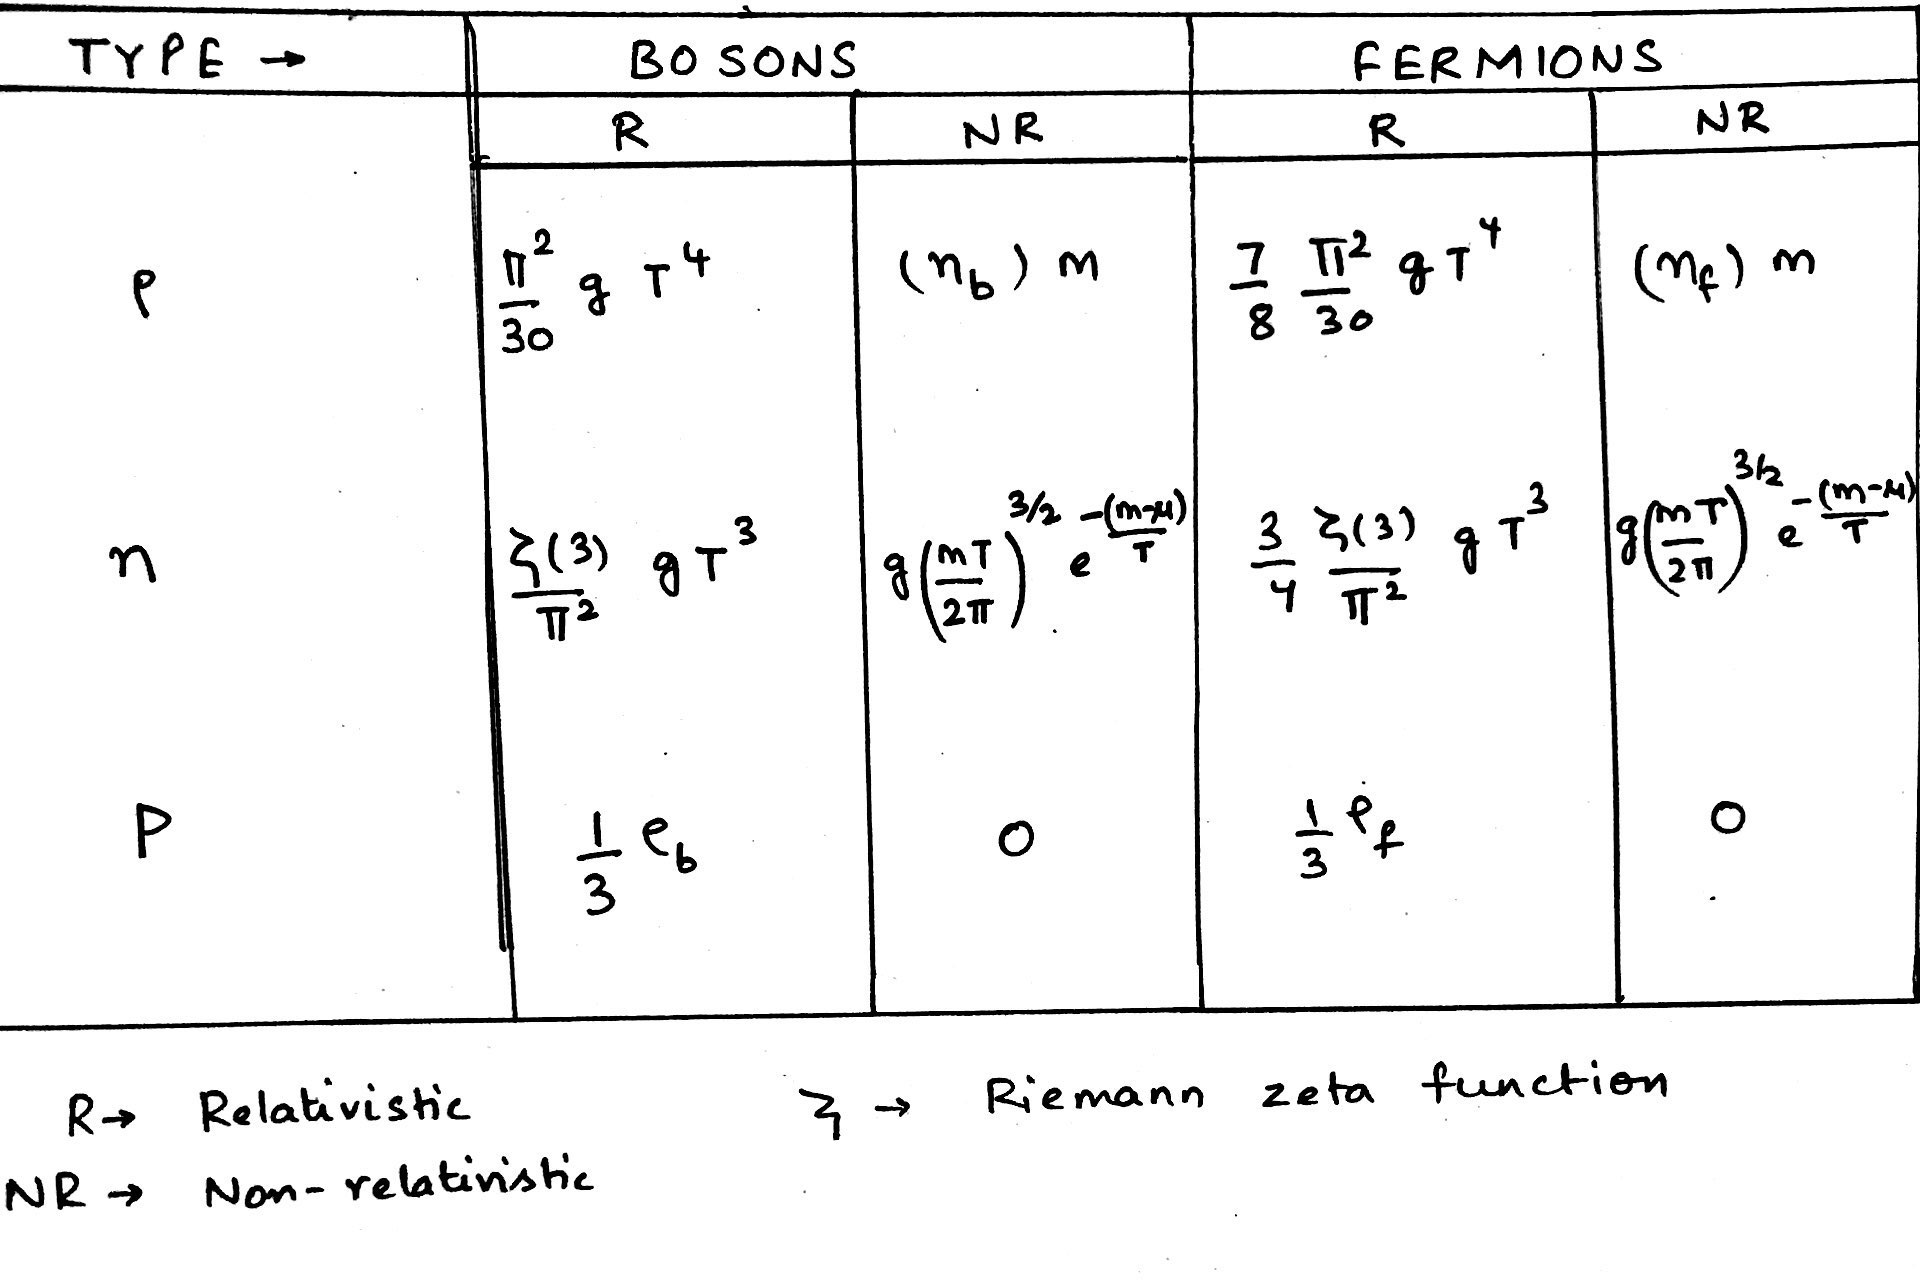
\includegraphics[width = 0.65\textwidth]{thermal_average_chart.jpg}
    \caption{Thermal average chart:  The table shows average energy density,number density and pressure calculated by evaluating the above integrals for bosons and fermions, when they are relativistic and non-relativistic }
    \label{fig:my_label}
\end{figure}
 \newline The dependence of each of the quantities on temperature can be understood as follows. For radiation/ relativistic species, the only quantity needed to describe the system in equilibrium is the temperature T. \textbf{Since energy density in radiation domination era goes as $\frac{1}{a^{4}}(t)$, we expect it to be $\propto T^{4}$}. For a non-relativistic species, there are two parameters- m and T and therefore the expression is somewhat non-trivial. The energy density is however equal to the product of number density and mass of the particle in the species as expected. We have introduced the chemical potential $\mu$ in the derivation above. Consider the reaction between 4 species 1,2,3,4 as shown below.
  \begin{center}
     \ce{ 1 + 2 <=> 3 + 4}
 \end{center} 
 The species are said to be in chemical equilibrium if the rate of forward reaction is equal to the rate of backward reaction. A useful quantity to define is the chemical potential $\mu$ given by the thermodynamic definition  $\mu = -T (\frac{\partial S}{\partial N}) $ at constant internal energy U, volume V. The condition for equilibrium will then be :
\begin{equation}
    \mu_{1} + \mu_{2} = \mu_{3} + \mu_{4}
\end{equation}
In the next section, we will study in detail how the condition (1.22) comes about. A species which is in both kinetic and chemical equilibrium is said to be in thermodynamic equilibrium.

relativistic matter: photons, neutrinos?
non-relativisitic : baryonic
\section{Entropy density}
In the previous section, we have seen how the total energy density(sum of energy densitites of all species) is nt a conserved quantity. Now, we'll see that the total entropy in the universe is a conserved quantity. These two statements might sound like violation of laws of thermodyanmics, where conservation of energy is valid and total entropy is always increasing. It can be explained as follows: ???
\\ The entropy density in a comoving volume is defined as 
\begin{equation}
    s = \frac{\rho + p}{T}
\end{equation}
The rate of change of total entropy density is therefore
\begin{equation}
    \frac{dS}{dt} =\frac{d(sa^3)}{dt} = a^3\frac{ds}{dt} + 3\dot{a}a^2s
\end{equation}
\begin{align}
    \frac{ds}{dt} &= \frac{\dot{\rho}+\dot{p}}{T} -\frac{\dot{T}}{T^2}(\rho + p)\\
    \dot{p} = \frac{1}{T}\frac{dp}{dT}\dot{T}
\end{align}
From first law of thermodynamiccs,
\begin{align}
    Tds &= d(\rho v) + pdv\\
    ds &= \frac{v}{T}\frac{d\rho}{dT}dT+ \frac{\rho + p}{T}dv 
\end{align}
Using the condition for ds to be exact differential, it can be shown that
\begin{align}
     \frac{dp}{dT} = \frac{\rho +p}{T}
\end{align}
Therefore,
\begin{equation}
    \frac{ds}{dt} = \frac{\dot{\rho}}{T} = \frac{-3\dot{a}}{Ta}(\rho+p)
\end{equation}
The last step is written using the continuity equation($ \dot{\rho} + 3H(\rho+p)=0$) which can just be derived by differentiating the first Friedmann equation and combining with he second. Subsituting back all the terms in $\frac{dS}{dt}$,
\begin{align}
    \frac{dS}{dt} &= -3\dot{a}a^2s+3\dot{a}a^2s \\
    \therefore  \frac{dS}{dt} &= 0
\end{align}
The total entropy is therefore conserved.
Time and temperature relation??
\section{The Boltzmann Equation}
The rate of change of abundance of any species is equal to the rate at which it is produced minus rate at which it is annihilated. This can be expressed as the boltzmann equation below:
\begin{equation}
  \frac{\Gamma}{H}  
\end{equation}
where the integrals over momentum
\newline explain rate eqn
\newline The equation can be understood as follows -  while the universe is expanding, there are two time scales : the reaction rate $\Gamma$ and rate of expansion H. When $\Gamma$ falls below H, the species do not have enough time to interact, as the distance between them changes faster than the universe is expanding(i.e; they are too far apart to find each other) and therefore they fall out of equilibrium. On the other hand, when $\Gamma$ is less than H, the species can interact and the right hand side of the \textbf{equation()} adjusts such that ultimately equilibrium is established. The former case when reaction rate drops below expansion rate is called "Freeze-out" or Decoupling and the abundance of the species at this freeze-out is known as relic abundance, since after decoupling, the comoving number density remains constant and the number density simply goes as $1/a^3$ due to increase in physical volume.
\newline Our goal now is to estimate roughly the temperature or time at which several reactions freeze out, and then go back to EQN() to solve for relic abundance  or equilibrium abundance.
\subsection{Neutrino decoupling}
Neutrinos interact only weakly with the rest of plasma through scattering processes such as \ce{\nu e^{-} -> \nu e^{-}} . The reaction rate for such reactions will be
\begin{equation}
    \Gamma  = n_{e}<\sigma v>  
\end{equation}
A reasonable assumption is to believe that the electrons are relativistic at the time of decoupling. If the temperature at freeze-out comes out to be > $m_{e}$, then our assumption is true. In that case, from Fig 1.1,
\begin{equation}
    n_{e} = \frac{3}{4}\frac{\zeta(3)}{\pi^3} 2 T^3 
\end{equation}
For weak interactions, the thermal averaged cross-section is given by
\begin{equation}
    \sigma  = \frac{g^4T^2}{M_{x}^{4}}
\end{equation}
where $g_{x}$ is the coupling constant, $M_{x}$ is the mass of mediator of the weak interaction. Dimensionally, cross-section should have the units of $[L]^{2}$. We know that the probability has to be dependent on the temperature($[L]^{-1}$) and mass of the mediator($[L]^{-1}$)\footnote{Detailed discussion on cross-section in next chapter}. Therefore, the expression for cross-section is dimensionally correct. Assuming scattering at relativistic velocities(v~1), and plugging in the above two equations, 
\begin{equation}
    \Gamma \propto T^5
\end{equation}
In radiation domination era, $ H^2 = 8\pi G\rho = \frac{T^4}{M_{pl}^{2}}$ where $M_{pl} = \sqrt{\frac{\hbar c}{8\pi G}}$  
\newline The ratio $\Gamma/ H$ is then 
\begin{equation}
    \frac{\Gamma}{H} \approx (\frac{T}{1Mev})^{3}
\end{equation}
Therefore, neutrino decoupling starts after a temperature around 1Mev. Our assumption that the electrons are relativistic during this period is also therefore true. 
\subsection{Matter-Radiation decoupling}
Baryonic matter is kept in equilibrium with radiation via electromagnetic interactions such as Thomson scattering($\gamma e^{-} -> \gamma e^{-}$). The rate of this reaction is clearly dependent on the number density of electrons. Shortly after the neutrinos decouple, the temperature drops below electron mass, making the backward reaction of the annihilation \ce{e^{-}e^{+} <-> \gamma \gamma} inefficient. This results in the annihilation of electrons, which decreases their number density, which in turn results in slowing down the rate of Thomson scattering, eventually leading to freeze-out. The electron-positron annihilation also heats up the photons, while the temperature of neutrinos simply falls as 1/a after decoupling and in fact, is lesser than the photon temperature.
\newline The reaction rate for Thomson scattering is 
\begin{equation*}
     \Gamma  = n_{e}<\sigma v> 
     \end{equation*}
\begin{equation}
    n_{e}  = 2(\frac{mT}{2\pi})^{3/2}\exp{-\frac{(m-\mu)}{T}}
\end{equation}
since the electrons are non-relativistic. The cross-section for electromagnetic interaction is given by
\begin{equation}
    \sigma = \frac{\alpha^2}{T^2}
\end{equation}
where $\alpha$ is the fine structure constant. Again, this can be verified dimensionally since $\sigma$ is $[L]^{2}$ and T is $[L]^{-1}$ and fine structure constant is dimensionless\footnote{Detailed discussion on cross-section in next chapter}.
\newline The ratio will be 
\begin{equation}
    \frac{\Gamma}{H} \propto T^{-5/2}exp{(1/T)}
\end{equation}
The temperature thus estimated will be around $T_{dec} \approx 0.3eV$.
\newline Note that this number is just an approximate value, in order to find the exact temperature, we need to find out the electron abundance from the Boltzmann equation/Saha equation, which will be done in the subsequent sections.
\subsection{Electron abundance}
\subsection{Nucleosynthesis}
We have seen that at temperatures of order of 1Mev, the neutrinos have already decoupled and electrons started annihilating to increase the number of photons. Meanwhile, the baryons(including protons, neutrons and light elements) are non-relativistic. The rate at which production of these elements takes place is evidently determined by the abundance of neutrons and protons. We make the following two assumptions to study nucleosynthesis. Firstly, we assume that there are the abundances of elements above Helium are negligible. The binding energy of Helium is the greatest among the light elements which makes it the most stable light element. Further fusion of Helium into  heavier elements therefore is not favourable. In stars, the triple alpha process results in the production of Carbon(\ce{^{4}He + ^{4}He + ^{4}He -> ^{12}C}) which cannot occur in the early universe because the abundance is not high enough for 3 Helium nuclei to find each other and fuse.  The other simplification is to consider that there are no light elements until the temperature falls below 0.1Mev and only free neutrons and protons exist. We will see that although the binding energy of elements like Deuterium is around 2.2Mev, due to the small baryon-to-photon ratio, the abundance isn't considerable until temperature falls below 0.1Mev.
\subsection{ Neutron abundance}
The reactions involving neutrons and protons can either be n-p inter-conversion via weak interactions(\ce{n e^{+} -> p $\bar{\nu}$}) or neutron decay(\ce{n -> p e^{-} $\bar{\nu}$}). The rate equation for neutron-proton inter-conversion will be -
\begin{equation}
    a^{-3}\frac{d(n_{n}a^{3})}{dt} = n_{l}^{0}<\sigma v>(\frac{n_{n}^{0}n_{p}}{n_{p}^{0}}-n_{n})
\end{equation}
where $n_{l}$ is the lepton number density and we have taken that the leptons are in equilibrium with the plasma as a whole and therefore $n_{l} = n_{l}^{0}$. For ease of calculation, we will express the above equation in terms of mass fraction, since they are independent of the scale factor. The neutron mass fraction is defined as 
\begin{equation}
    X_{n} = \frac{n_{n}}{n_{n}+n_{p}}
\end{equation}
Eqn(1.32) then becomes 
\begin{equation}
    1
\end{equation}


\section{WIMP freeze out}
*introduction about WIMP* \\
We will assume that WIMP is a majorana particle, meaning it is its own anti-particle(therefore, g =2), that it is thermally produced and has mass in the order of GeV. The GeV mass range is a good guess from cosmological point of view, because once temperature falls below the mass~ GeV, the dark matter annihilation becomes more efficient, leading to decrease in their number density until they couldn't anymore find another particle to annihilate with, causing freeze-out. Therefore, at the end of freeze-out, the WIMP particles are non-relativistic, which is required for the formation of structures in the universe later on. We will consider the main interaction to be annihilation of WIMPs giving rise to massless leptons as follows.
\begin{equation}
        X + X -> l + l
\end{equation}
The Boltzmann equation for the above reaction is :
\begin{equation}
    \frac{1}{a^3}\frac{d(na^3)}{dt} = \frac{dn}{dt} + 3Hn = <\sigma v> (n_{eq}^2 - n^2)
\end{equation}
where n is the physical number density of dark matter particles(will bea function of temperature,mass as shown in  Fig1.1) and we have considered that the leptons are always in thermal equilibrium with the rest of the plasma leading to $n_{l}^{(0)} = n_{l}$. As we see in Eqn(1.36), when the left hand side dominates over the expansion rate, if $n >  n_{eq}$, the rate of change is negative, so that the number density decreases and finally reaches its equilibrium value. Similarly, when $n < n_{eq}$, the rate of change of number density is positive, and the number density keeps increasing till $n = n_{eq}$ and the rate is equal to zero.\\ In the other case, when the reaction rate is lesser than the Hubble expansion rate, we simply have
\begin{equation*}
     \frac{1}{a^3}\frac{d(na^3)}{dt} = 0
\end{equation*}
which implies the comoving number density is conserved. We then say that the dark matter has decoupled or "frozen-out". Using the fact that the total comoving entropy(S = s$a^3$) is conserved, we make a change of variable in the above equation and define Y as
\begin{equation}
     Y  = n/s
\end{equation}
and 
\begin{equation}
    x = m/T
\end{equation}
The differential equation will now be 
\begin{equation}
    \frac{dY}{dx} = \frac{s<\sigma v>}{xH}(Y_{eq}^2 - Y^2)
\end{equation}
where we have used the fact aT = const. in the radiation domination era and used the chain rule to get $\frac{dx}{dt}$.\\ The above equation has to be solved numerically to get exact solution but can be simplified to solve analytically by dealing it in two regimes, before the freeze-out until Y drops significantly from $Y_{eq}$ and after the freeze-out until today to get the abundance today.\\ In the latter case, $ Y >> Y_{eq}$ and the equation becomes
\begin{equation}
    \frac{dY}{dx}  = \frac{\lambda}{x^2}(- Y^2) 
\end{equation}
where $\lambda = s<\sigma v>/H(m)$. Integrating the equation between $Y_{f}$ and $Y_{\infty}$, at freeze-out and infinity respectively, we get
\begin{equation}
    \frac{1}{Y_{f}} - \frac{1}{Y_{\infty}} = -\frac{\lambda}{x_{f}}
\end{equation}
assuming $x_{\infty} \approx 0$. Typically, Y at freeze-out is much larger than Y at infinity, so we can approximate the above expression to get $Y_{\infty}$ as 
\begin{equation}
    Y_{\infty} \approx \frac{x_{f}}{\lambda}
\end{equation}
The abundance of dark matter today will be given by 
\begin{equation}
    \rho_{X}^{(0)} = n_{X}^{(0)}*m_{X} = Y_{\infty}*s_{\infty}*m_{X}
\end{equation}
where $s_{\infty} = \frac{2\pi^2}{45}g_{s}T_{\infty}^3 $ \\
Getting $<\sigma v>$ for dm-dm annihilation ?
\chapter{Elementary Particle Physics}
\section{Feynman diagrams}
In the previous chapter, we have seen that the deciding factor as to whether a chemical reaction or an interaction takes place in the expanding universe is dependent on whether the rate $\Gamma$  >/< H. We have also seen that for the forward reaction \ce{A+ B-> C+D}
\begin{equation}
    \Gamma \propto n_{B}<\sigma v>
\end{equation}
where the cross-section $\sigma$ is dependent on the type of interaction. We'll consider the standard model interactions- weak, strong and electromagnetic. \\
Feynman diagrams provide a simple way to represent the interaction and following the prescribed rules, it is easy to write the scattering amplitudes. For example, consider the scattering of $e^{-}$, $e^{+}$.
\begin{equation*}
    e^{+} + e^{-} -> e^{+} + e^{-}
\end{equation*}
 The interaction of course is electromagnetic. In our diagram, time always flows from left to right. Each vortex represents the interaction between the particles/ anti-particles. Incoming particles and outgoing anti-particles are represented by arrows into the vertex and vice-versa. At all times, all conservation laws apply i.e; we have the charge conservation, energy-momentum conservation, lepton number, color conservation. Keeping in view these, there can be three-ways to draw the Feynman diagram.
\begin{itemize}
    \item s-channel diagram:\par 
    \begin{minipage}{\linewidth}
        \centering
        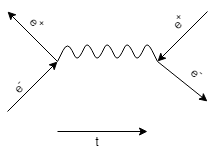
\includegraphics[width = 5cm]{s_feynman_diag.png}
        \label{fig:my_label}
    \end{minipage}
    \\ The wiggly line is the virtual particle carrying the force - a photon in this case for the electromagnetic interaction. The momentum carried by the photon is
    \begin{equation}
        p_{\gamma} = p1 -p2 = p3 -p4
    \end{equation}
    where p1, p2 are momentum of incoming $e^{-}$ and $e^{+}$ and p3, p4 for the outgoing $e^{-}$ and $e^{+}$.
    \item t- channel diagram:\par 
    \begin{minipage}{\linewidth}
        \centering
        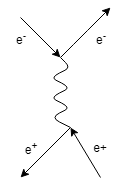
\includegraphics[width =4cm]{t_feynman_chan.png}
        \label{fig:my_label}
    \end{minipage}
    \\ The momentum of photon in this case would be :
    \begin{equation}
        p_{\gamma} = p1 -p3 = p2 -p4
    \end{equation}
    \item u-channel diagram: It is not possible to have a u-channel diagram in this case because it'll violate charge conservation. In general, the Mandelstam variable for u-channel is 
    \begin{equation}
        u = (p1-p4)^2 = (p3-p2)^2
    \end{equation}

     %\begin{minipage}{\linewidth}
      %  \centering
       % 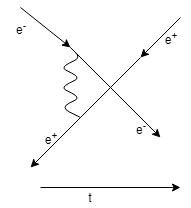
\includegraphics[width = 5cm]{t_channel_feynman_daiag.png}
        %\label{fig:my_label}
    %\end{minipage}
    %\\ The momentum of photon is :
    %\begin{equation}
     %    p_{\gamma} = p1 -p4 = p2 -p3
    %\end{equation}
    \\ Observe that in addition to knowing p3,p4, we know that final products are distinguishable in the reaction considered, so it's enough if we consider t-channel diagram alone??
\end{itemize}
\section{Scattering cross-section}
Scattering cross-section is the effective area that a particle finds available to interact with the other.The scattering cross section is propto?? the scattering amplitude, which can be written from the Feynman diagrams. We'll look at the scattering amplitude and cross-section for a few of the reactions we encountered in the last chapter.
\subsection{Neutrino scattering}
As we have seen previously, neutrinos decouple when the process of scattering between neutrino and electron becomes inefficient. The interaction has to be weak. 
\begin{equation*}
    \nu + e^{-} ->  \nu + e^{-}
\end{equation*}
For this reaction, we can draw both t and u channel diagrams but not s-channel because lepton number conservation will be violated.\par
\begin{minipage}{\linewidth}
    \centering
    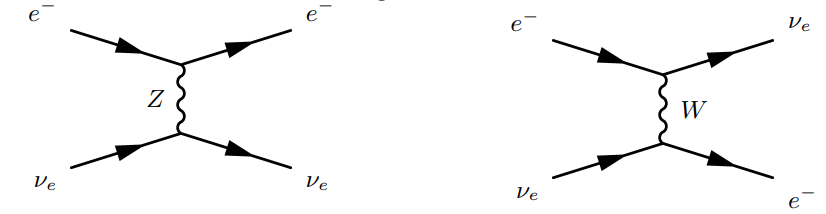
\includegraphics[width = 10cm]{wz.png}
   % \caption{Caption}
    %\label{fig:my_label}
\end{minipage}
The scattering amplitude for t-channel would be :
\begin{equation}
    |M1| \propto \frac{1}{p_{z}^2-m_{z}^2}
\end{equation}
and for u-channel :
\begin{equation}
    |M2| \propto \frac{1}{p_{w}^2-m_{w}^2}
\end{equation}
The total scattering amplitude is sum of the amplitudes and scattering amplitude is proportional to the square of the sum.
\begin{align}
    |M|^2 &= |M1+M2|^2 = |M1|^2 + |M2|^2 + |M1(M2)*| + |(M1)*M2|\\
    \sigma & \propto |M|^2
\end{align}
\\ DOUBT !!!!!!!!!!!!!!!!
In general, we can say from dimensional analysis that since cross-section is $[L]^2$, we know that it should be $ [M]^{-2}$ and for weak interaction, we have massive mediators and therefore E$\approx$ M. There are two vertices and therefore scattering amplitude has $g^2$ and $\sigma \propto M^2 \propto g^4$. Therefore,
\begin{equation}
    \sigma \approx \frac{g^4}{M2} \approx \frac{g^4}{E^2} \approx \frac{g^4}{T^2}
\end{equation}
The last step is in the context of early universe where T is the temperature of the thermal bath.
\subsection{Thomson scattering}
%We've seen that when the temperature of universe fell below $m_{e}$, the electron-positron annihilation froze-out and the whole energy was transferred to photons.
Should it be discussed???
We've seen that the matter-radiation decoupling happened when the rate of Thomson scattering fell below the Hubble rate. The scattering cross-section can be derived from classical electrodynamics as well. Here,we'll look at the scattering cross-section obtained by the Feynman diagram. For
\begin{equation}
 \gamma e^{-} -> \gamma e^{-}   
\end{equation}

\subsection{Dark matter annihilation}
Consider the reaction
\begin{equation*}
    X + X -> Y +Y
\end{equation*}
The interaction part of the Lagrangian density() should look something like:
\begin{equation}
    L_{int} = c XXYY
\end{equation}
where c is the coupling constant and therefore there is no interaction when c = 0. The scattering amplitude must therefore include the coupling constant(c) for each interaction i.e; at each vertex. The other term in scattering amplitude is 
\begin{equation}
    \frac{1}{p^2-m^2}
\end{equation}
where p,m are that of the virtual particle. If it's a massless particle, $|M| \propto p^{-2}$. The momentum of mediator is the difference between the momentum of incoming particles, and they obey the on-shell condition.
%Therefore, for a massive WIMP, it's energy is almost equal to it's mass. 
\\ Cross-section has dimensions of $[L]^{2}$ which is $\propto m^{-2}$. So, we expect is to be inversely proportional to the mass of incoming particle or more generally like $E^2/m^4$ which in the massive particle limit gives the same term.
\\ Feynman diagram possible for dm-dm annihilation will be s-channel.
\begin{figure}
    \centering
    \includegraphics[width = 5cm]{}
    \caption{Caption}
    \label{fig:my_label}
\end{figure}
%\section{Neutrino Oscillations}
\chapter{Astroparticle Physics}
\section{Dark Matter: Introduction}
 Evidence: Dark matter was introduced by Zwicky\footnote{} as the "invisible" matter which was required if galaxy clusters were to be virialised.He found that the total mass of all luminous matter in the Coma cluster wouldn't be enough for the cluster to be stable,by applying the virial theorem. While it is also possible to think that the Coma cluster might not have been virialised at the time, or that there is non-luminous baryonic matter that we didn't account for, these reasons were eliminated using other techniques?. Typically, for a galaxy, as the density of matter decreases as we go away from the centre, and therefore we expect the distant stars to have lower orbital velocities. However,the galaxy rotation curves obtained by Vera Rubin indicated that velocity curve is not decreasing but instead remained flat as distance from the galaxy centre increased. One resolution provided was that the mass density doesn't decrease as we move away and that there is a lot of dark matter in the outskirts. There have been other ways tried out in this case as well, the most succesful being Modified Newtonian Dynamics or MOND. But the strongest evidence for dark matter comes from the formation of large scale structure in the universe. The existence of cold dark matter, as we have already seen, is a major feature of the Standard model of cosmology. The argument is that if the dark matter was not cold(i.e; T>>m or relativistic), it wouldn't have been possible for the structures to form, since the relativistic particles free stream and smear the density perturbations\footnote{Details in Additional topics}.
\\ Particle nature --?? 

\subsection{Direct detection}
???
Collision of dark matter with standard model particles.
\subsection{Indirect detection}
The idea of indirect detection is not to detect dark matter directly, but to look for the standard model particles that might have been the end products of dark matter processes. In particular, we'll be looking at dark matter-dark matter annihilation($\chi +\chi -> SM +SM$) and dark matter decay($\chi -> SM$).
 The important question is where to look for the products. We may want to look at places where the rate of the process to occur is high for eg. at the center of the halo i.e; center of the galaxy but it's not a clean source since a lot of other processes are going on as well. Therefore, the right parameter would be the rate at which particles are received per unit solid angle at the detector, which is dependent on :
\begin{equation}
    \frac{1}{r^2d\Omega}\frac{dN}{dt} = \int n_{x}(n_{x}<\sigma v>)f_{SM}\frac{dV}{L^2} 
\end{equation}
\par where the first two terms explain the rate of annihilation while $f_{SM}$ contains all the particle physics of SM products and the integration is over the whole source volume. Therefore, the rate is 
\begin{equation}
     \approx \frac{\rho^2 V}{L}\frac{f_{SM}<\sigma v>}{m^2}
\end{equation}
We can see that our detection chances increase when we look at sources 
\chapter{Additional topics}
\section{Liouville operator}
\section{Structure formation}

%\subsection{Energy loss argument}
%\section{Neutrinos}
%%%%%%%%%%%%%%%%%%%%%%%%%%%%%%%%%%%%%%%%%%%%%%%%%%%%%%%%%%%%%%%%%%%%%%%%%%%%%%%
\section{Appendix}
\subsection{ Average pressure of a thermal distribution}
\subsection{Thermal average inegrals, gamma functions}
\begin{thebibliography}{99}
%%%%%%%%%%%%%%%%%%%%%%%%%%%%%%%%%%%%%%%%%%%%%%%%%%%%%%%%%%%%%%%%%%%%%%%%%%%%%%%
\bibitem{[1]} See, http://www.sdss.org/science/orangepie/
\bibitem{[2]} See, https://map.gsfc.nasa.gov/media/121238/index.html
\bibitem{[3]} Image credit : Aseem Paranjape, IUCAA VSP 2017 lectures
\bibitem{4} See, http://www.damtp.cam.ac.uk/user/db275/Cosmology/Lectures.pdf
\bibitem{0904.4584}
L. Sriramkumar.
\newblock An introduction to inflation and cosmological perturbation theory, 2009;
\newblock arXiv:0904.4584
\bibitem{[5]} Dodelson, Scott. Modern Cosmology. Academic Press, 2003.
\bibitem{}Schneider, P. Extragalactic Astronomy and Cosmology: an Introduction. Springer, 2006.
%\bibitem{[6]} https://arxiv.org/pdf/0904.4584.pdf
%\bibitem{[7]} http://www.damtp.cam.ac.uk/user/db275/Cosmology/Chapter4.pdf
%\bibitem{[8]}  Galaxy formation \& Evolution by Mo, White,
Bosch
\bibitem{}Mo, Houjun, et al. Galaxy Formation and Evolution. Cambridge University Press, 2010.
\bibitem{[9]}M. Tegmark et al, Astrophys. J. 606, 702 (2004).
%See, {\tt http://magnum.anu.edu.au/~TDFgg/}.
%%%%%%%%%%%%%%%%%%%%%%%%%%%%%%%%%%%%%%%%%%%%%%%%%%%%%%%%%%%%%%%%%%%%%%%%%%%%%%%%
%\bibitem{sdss}
%See, {\tt http://www.sdss.org/}.
%%%%%%%%%%%%%%%%%%%%%%%%%%%%%%%%%%%%%%%%%%%%%%%%%%%%%%%%%%%%%%%%%%%%%%%
%%%%%%%%

\end{thebibliography}
%%%%%%%%%%%%%%%%%%%%%%%%%%%%%%%%%%%%%%%%%%%%%%%%%%%%%%%%%%%%%%%%%%%%%%%%%%%%%%%

%\end{comment}
\end{document}